\chapter{Methods}
\label{chapter2}

% Have a section for each paper
% Have lot's of graphs and images

% short summary of your method, 1 to 2 paragraphs
% the three sections on the three papers
% implementation details, for example, you can break it down into steps like how you did on reddit
% ps: use as many figure to show your work as possible
% figures include: at least one illustration on how your method work and as many figures on the ocean as possible

\section{IFFT}
\subsection{Butterfly Texture \ref{fig:ifft_algorithm}}
Firstlly we only intrested in IFFT algorithm and we will not use FFT.
To perform IFFT we going to produce so called butterfly texture by \cite[Fl{\"u}gge Fynn-Jorin]{flugge2017}.
This texture has width of $(log_2(n)$ and height of $n$ and is precomputed and stored inside the GPU memory once, unless the data size changes. This is 4 chanel texture $(W_r, W_i, y_t, y_b)$,
where $W_r$ and $W_i$ are real and imaginary parts of the twiddle factor, $y_t$ and $y_b$ are top and bottom butterfly indices as shown in \ref{fig:butterfly_diagram}.

In butterfly texture coordinate x represents a stage \ref{fig:8_butterfly_diagram}, while each y represents a butterfly operation between two data points $y_t$ and $y_b$.

In the first stage we assign $y_t$ and $y_b$ in bit reversed order, on the other stages:
\begin{itemize}
    \item If the butterfly wing is top half
    \begin{equation}
        \begin{split}
            y_t &= y_{\text{current}} \\
            y_b &= y_{\text{current}} + 2^{\text{stage}}
        \end{split}
    \end{equation}
    \item If the butterfly wing is bottom half
    \begin{equation}
        \begin{split}
            y_t &= y_{\text{current}} - 2^{\text{stage}} \\
            y_b &= y_{\text{current}}
        \end{split}
    \end{equation}
\end{itemize}
We can determine if the wing is upper or lower half:
\begin{equation}
    \text{wing} = y_{\text{current}} \bmod 2^{(\text{stage} + 1)}
\end{equation}
Lastlly we need to calculate twiddle factors:
\begin{equation}
    \begin{split}
        k &= (y_{\text{current}} \cdot n / 2^{\text{stage} + 1}) \bmod n \\
        W &= \exp(-2\pi i k / n)
    \end{split}
\end{equation}

\subsection{Performing IFFT}
Currentlly our data is stored in 2D texture. While this algorithm only accepts 1D data. Therefore, we need to perform 1D IFFT on each row "horizontally" and then on each column "vertically" \ref{fig:ifft_algorithm}.
By following pseudocode from \cite{flugge2017} we can perform IFFT in 2D:

\begin{lstlisting}[caption={Horizontal Butterfly Operation}, frame=single, numberstyle=\small\color{gray}, captionpos=b]
    float4 butterflyData = ButterflyTexture[float2(Stage, id.x)];
    const float2 twiddle = butterflyData.xy;
    // fetch top butterfly input sample
    topSignal = PingPong0[float2(butterflyData.z, id.y)].xy;
    // fetch bottom butterfly input sample
    bottomSignal = PingPong0[float2(butterflyData.w, id.y)].xy;
    // perform butterfly operation
    h = topSignal + ComplexMult(twiddle, bottomSignal);
\end{lstlisting}

Notice that we are using ping-pong buffers to store intermediate results, as we need to perform multiple IFFT passes, in total $log_2(n)$ passes.
After we perform IFFT on each row, we need to perform for each column:
\begin{lstlisting}[caption={Vertical Butterfly Operation}, frame=single, numberstyle=\small\color{gray}, captionpos=b]
    float4 butterflyData = ButterflyTexture[float2(Stage, id.y)];
    const float2 twiddle = butterflyData.xy;
    // fetch top butterfly input sample
    topSignal = PingPong0[float2(id.x, butterflyData.z)].xy;
    // fetch bottom butterfly input sample
    bottomSignal = PingPong0[float2(id.x, butterflyData.w)].xy;
    // perform butterfly operation
    h = topSignal + ComplexMult(twiddle, bottomSignal);
\end{lstlisting}

\subsection*{Permutation}
Lastlly, our data needs to be permuted as you will see later our data is offseted:
\begin{equation}
    [\text{freq} (-N / 2), \text{ ...}, \text{ freq} (-1), \text{ freq} (0), \text{ freq} (1), \text{ ...}, \text{ freq} (N / 2 - 1)]
\end{equation}
While, our IFFT algorithm expected data to be in the following order:
\begin{equation}
    [\text{freq} (0), \text{ freq} (1), \text{ ...}, \text{ freq}(N - 1)]
\end{equation}
This causes our data to flip sign in grid like pattern therefore we need to permute our data:
\begin{lstlisting}[caption={Data Permutation \cite{flugge2017} }, frame=single, numberstyle=\small\color{gray}, captionpos=b]
    float perms[] = {-1, 1};
    uint index = int((id.x + id.y) % 2);
    float perm = perms[index];
    float h = perm * PingPong1[id.xy].x;
    
    PingPong0[id.xy] = float4(h, h, h, 1);
\end{lstlisting}

\begin{minipage}{1\textwidth}
    \centering
    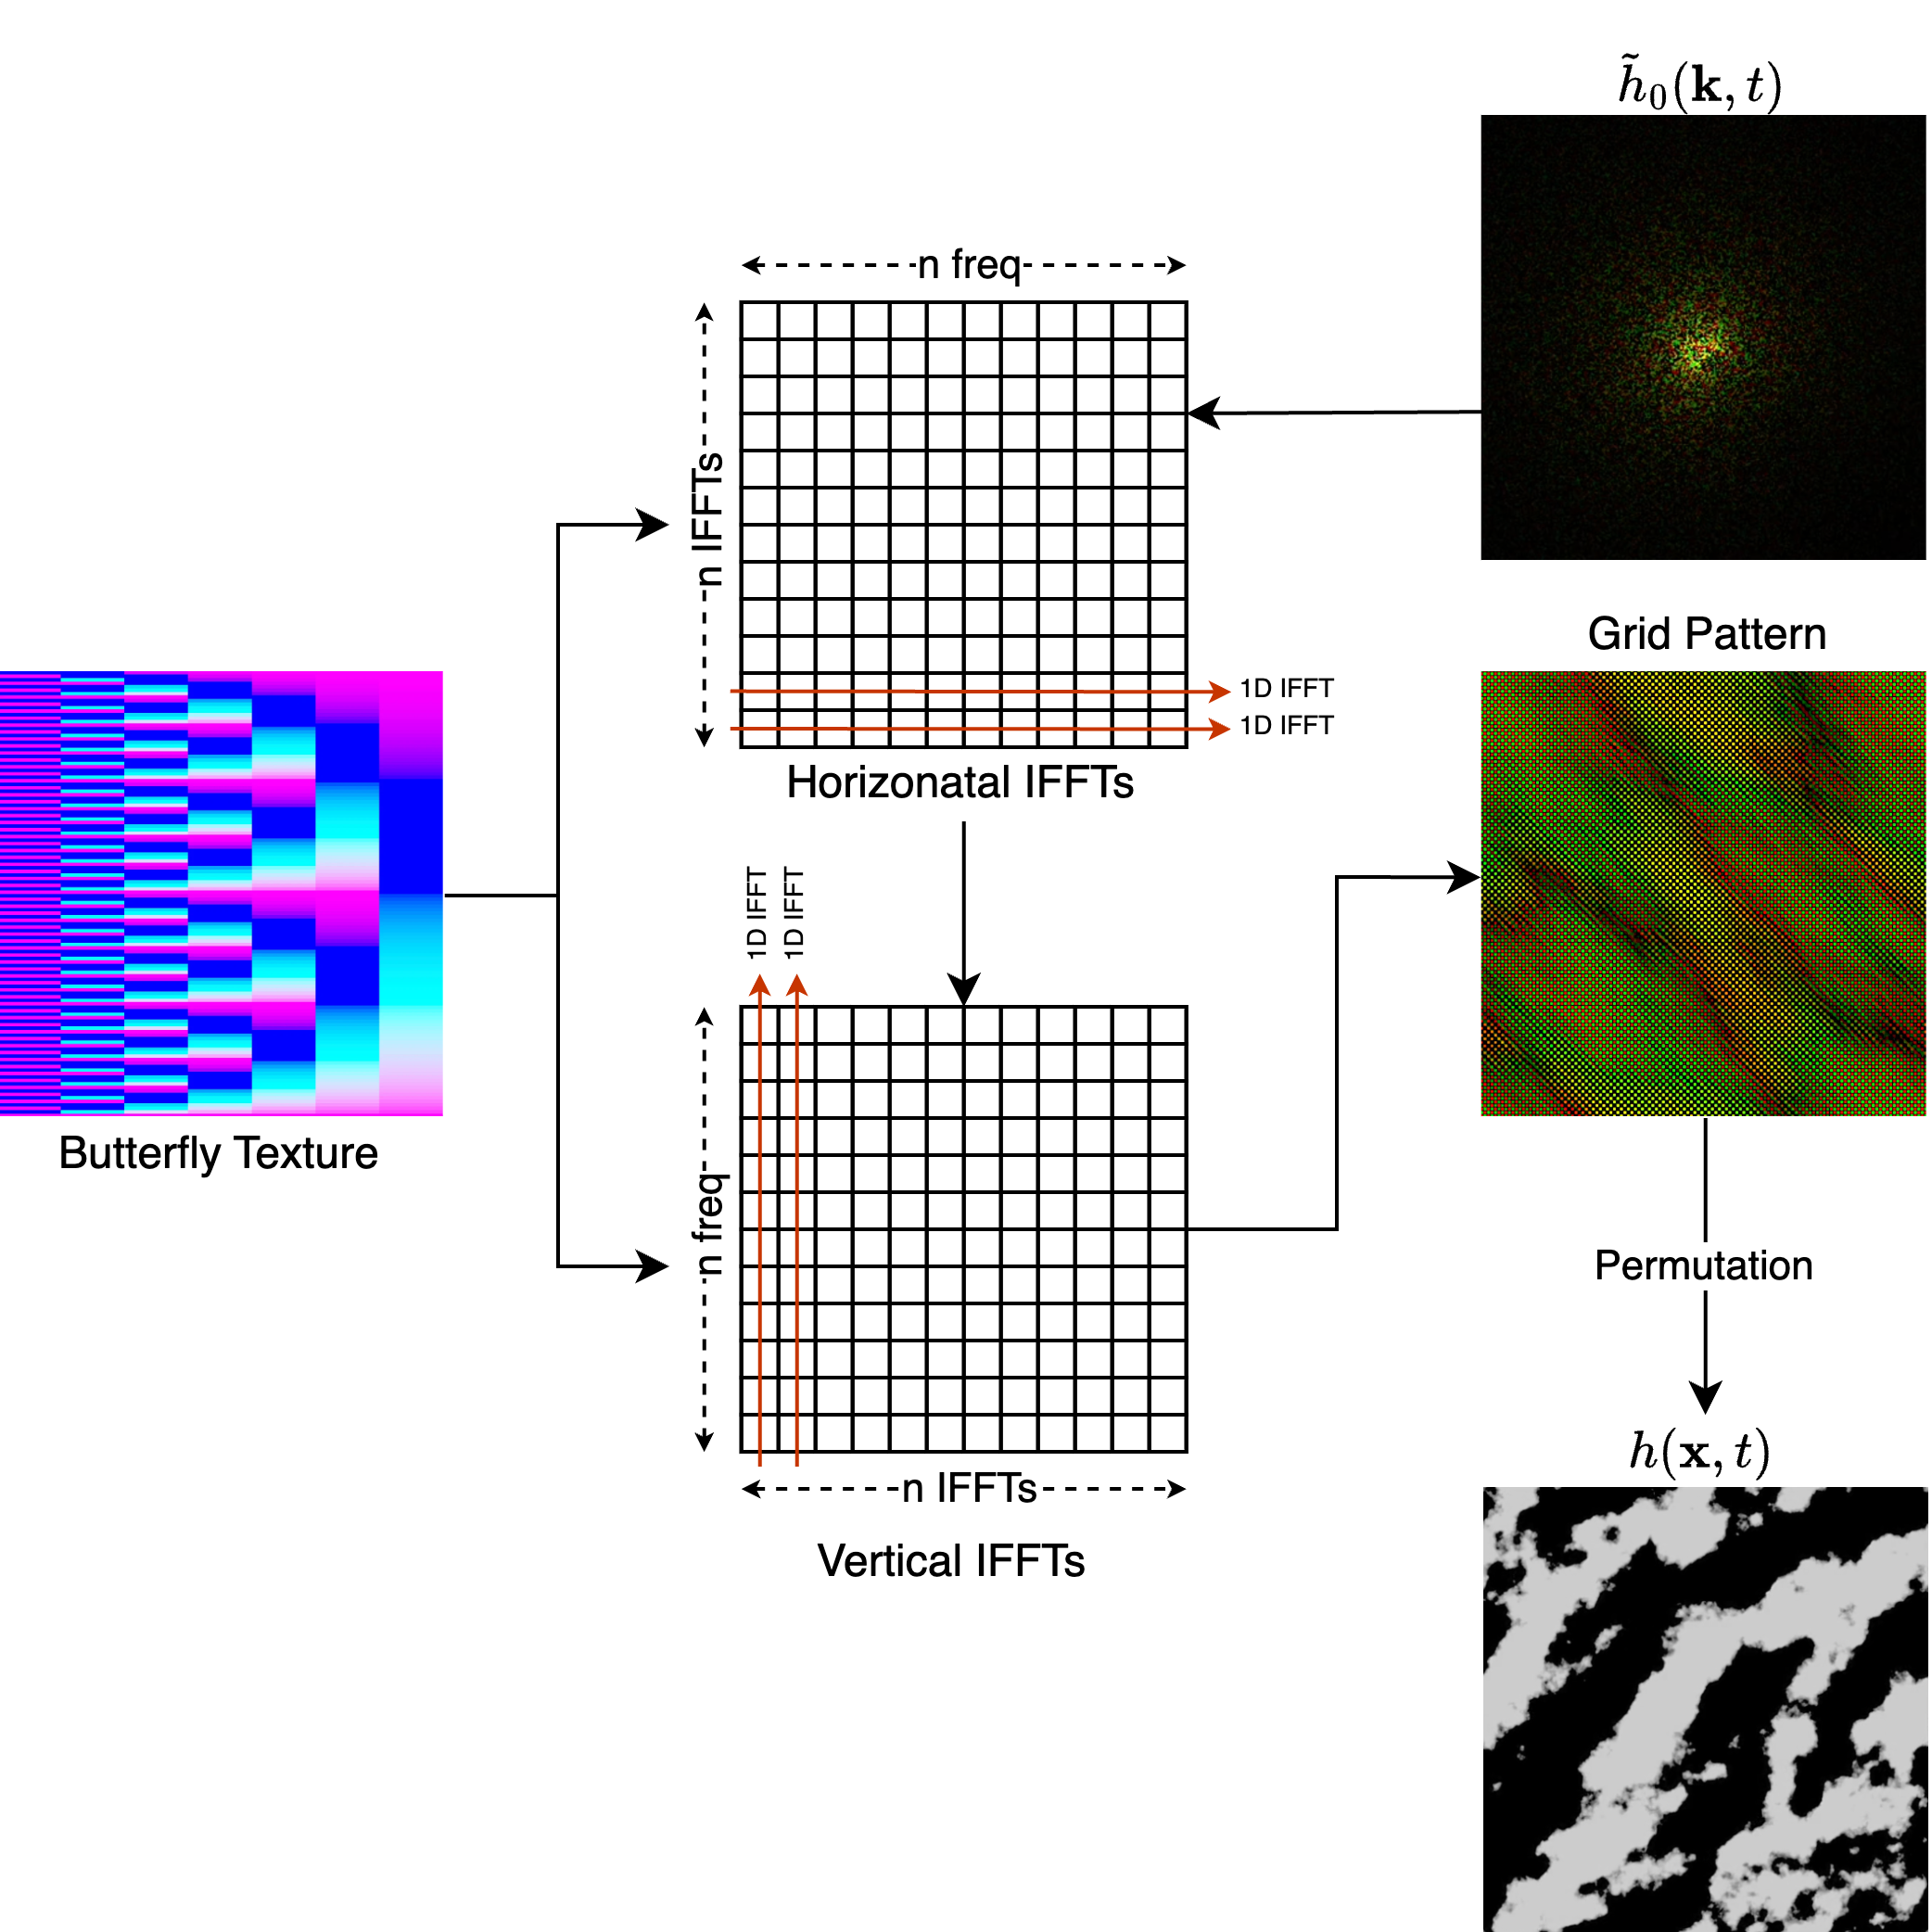
\includegraphics[width=0.7\textwidth]{"images/ifft_algorithm.png"}
    \captionof{figure}{IFFT Algorithm}
    \label{fig:ifft_algorithm}
\end{minipage}

\section{Ocean Geometry}
\subsection{Spectrum Generation}

% % Table
% \begin{table}
%     \centering
%     \begin{tabular}{|c|c|c|}
%         \hline
%         \textbf{Symbol} & \textbf{Parameter} & \textbf{Expression} \\
%         \hline
%         $\mathbf{k}$ & wave length &  \\
%         \hline
%         $\omega$ & dispertion relationship & x \\
%         \hline
%     \end{tabular}
%     \caption{Deffinition Table}
%     \label{table:deffinition_table}
% \end{table}

Spectrums are responsable for whole look of the ocean. It's importatnt to pick the one that is based on real world data to make our ocean look realistic.
Initialy, Tessendorf spectrum \ref{eq:tessendorf_spectrum} was implemented as it was straight forward to implement. However, it didn't produce satisfying results, as waves didn't seem to transfer energy in convincing way, waves didn't seem to follow wave direction and it was hard to have artistic control over the ocean.

\begin{minipage}{1\textwidth}
    \centering
    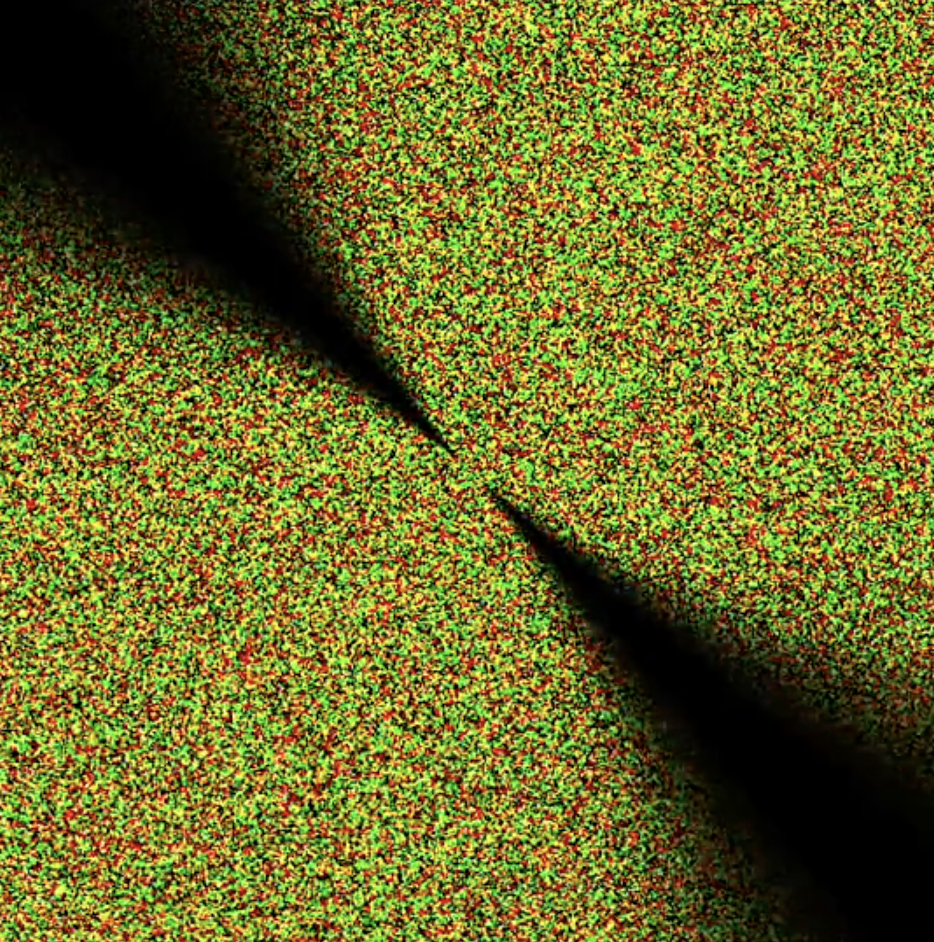
\includegraphics[width=0.4\textwidth]{"images/phillips_spectrum.png"}
    \captionof{figure}{Jerry Tessendorf's Spectrum}
    \label{fig:phillips_spectrum}
\end{minipage}

Therefore, TMA spectrum \ref{eq:tma_spectrum_k} was implemented. This spectrum resulted in more relistic looking ocean with intuitive controls: fetch, wind speed, wind angle, depth. Moreover, it didn't require any efort to make the ocean look relistic and it just worked out of the box.
\begin{minipage}{1\textwidth}
    \centering
    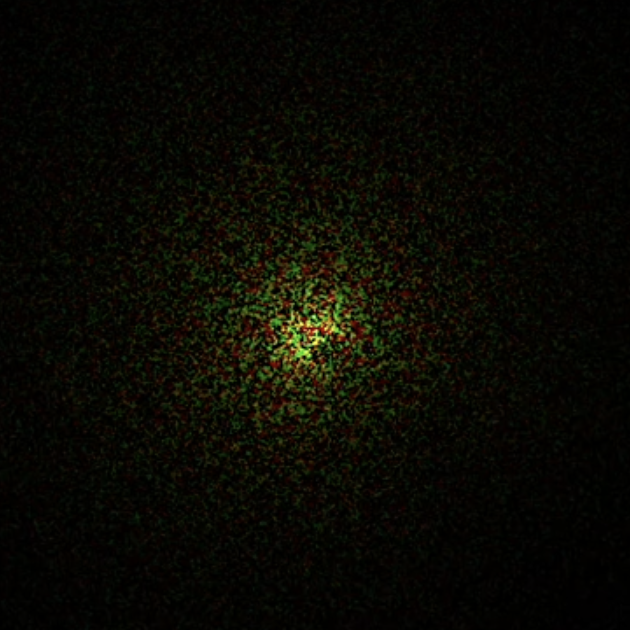
\includegraphics[width=0.40\textwidth]{"images/tma_spectrum.png"}
    \captionof{figure}{TMA spectrum, Frequency Domain \\ (100x for better visibility)}
    \label{fig:tma_spectrum}
\end{minipage}

\subsection{Height Map Generation}

To generate height map, firstlly we need to have fourier amplitudes as shown in \ref{eq:fouier_amplitudes}, where $P_h$ is TMA Spectrum $S_{TMA}(\mathbf{k})$.
For the next step we need to add fourier amplitude and it's complex conjugate to produce "produce waves towards and against the wave direction when propagating"\cite{horvath2015}.
In our luck we don't need to recalculate complex conjugate as fourier series are symetric, so we can just mirror the amplitudes:
\begin{equation}
    \tilde{h}^{*}_0 = T_{h_0}(x^{*}, y^{*})
\end{equation}
where $T_{h_0}(x, y)$ is fourier amplitude in precomputed texture at $x^{*} = (n - x) \text{ mod } n$, $y^{*} = (n - y) \text{ mod } n$, $(x, y)$ is current position in the texture.

By having combined amplitudes \ref{eq:combined_amplitudes} we can perform IFFT as shown in \ref{fig:ifft_algorithm} to produce height map.
\begin{minipage}{1\textwidth}
    \centering
    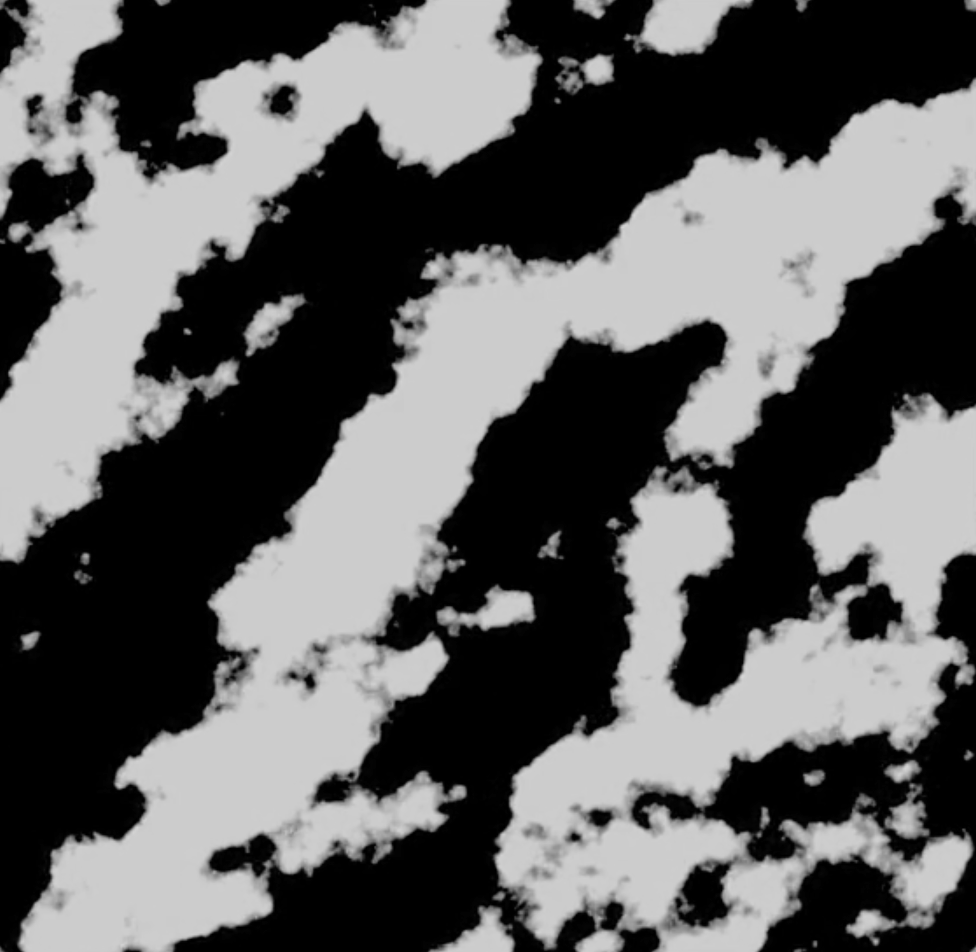
\includegraphics[width=0.40\textwidth]{"images/tma_height.png"}
    \captionof{figure}{Height Map using $S_{\text{TMA}}$}
    \label{fig:tma_height_map}
\end{minipage}

\subsection{Normal Map Generation}
Latter we will need extra information about the ocean to calculate ocean shading. Therefore, we need to calculate normal map. Normal map is perpendicular direction to the surface of the ocean.
To calculate normal map we need to calculate gradient, which is derivative of the height map. According to \cite{tessendorf2004} the derivative is:
\begin{equation}
    \epsilon(\textbf{x}, t) = i\textbf{k} \tilde{h}(\textbf{k}, t)
\end{equation}
Then we need to perform IFFT \ref{fig:ifft_algorithm} to get normal map in the time domain.

\begin{minipage}{1\textwidth}
    \centering
    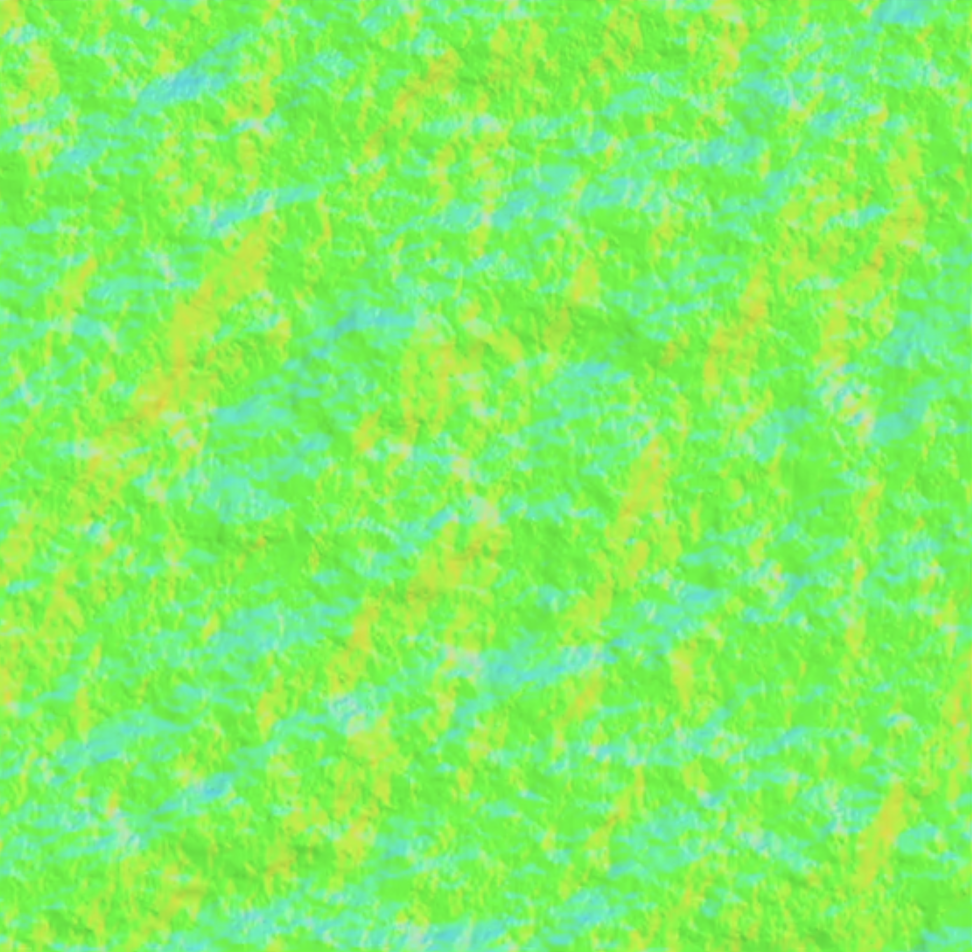
\includegraphics[width=0.40\textwidth]{"images/tma_normal.png"}
    \captionof{figure}{Normal Map using $S_{\text{TMA}}$}
    \label{fig:tma_normal_map}
\end{minipage}

\subsection{Choppy Waves}
Currentlly, when rendering ocean it looks too smooth \ref{fig:ocean_no_choppy} and lacks choppiness.

\begin{minipage}{1\textwidth}
    \centering
    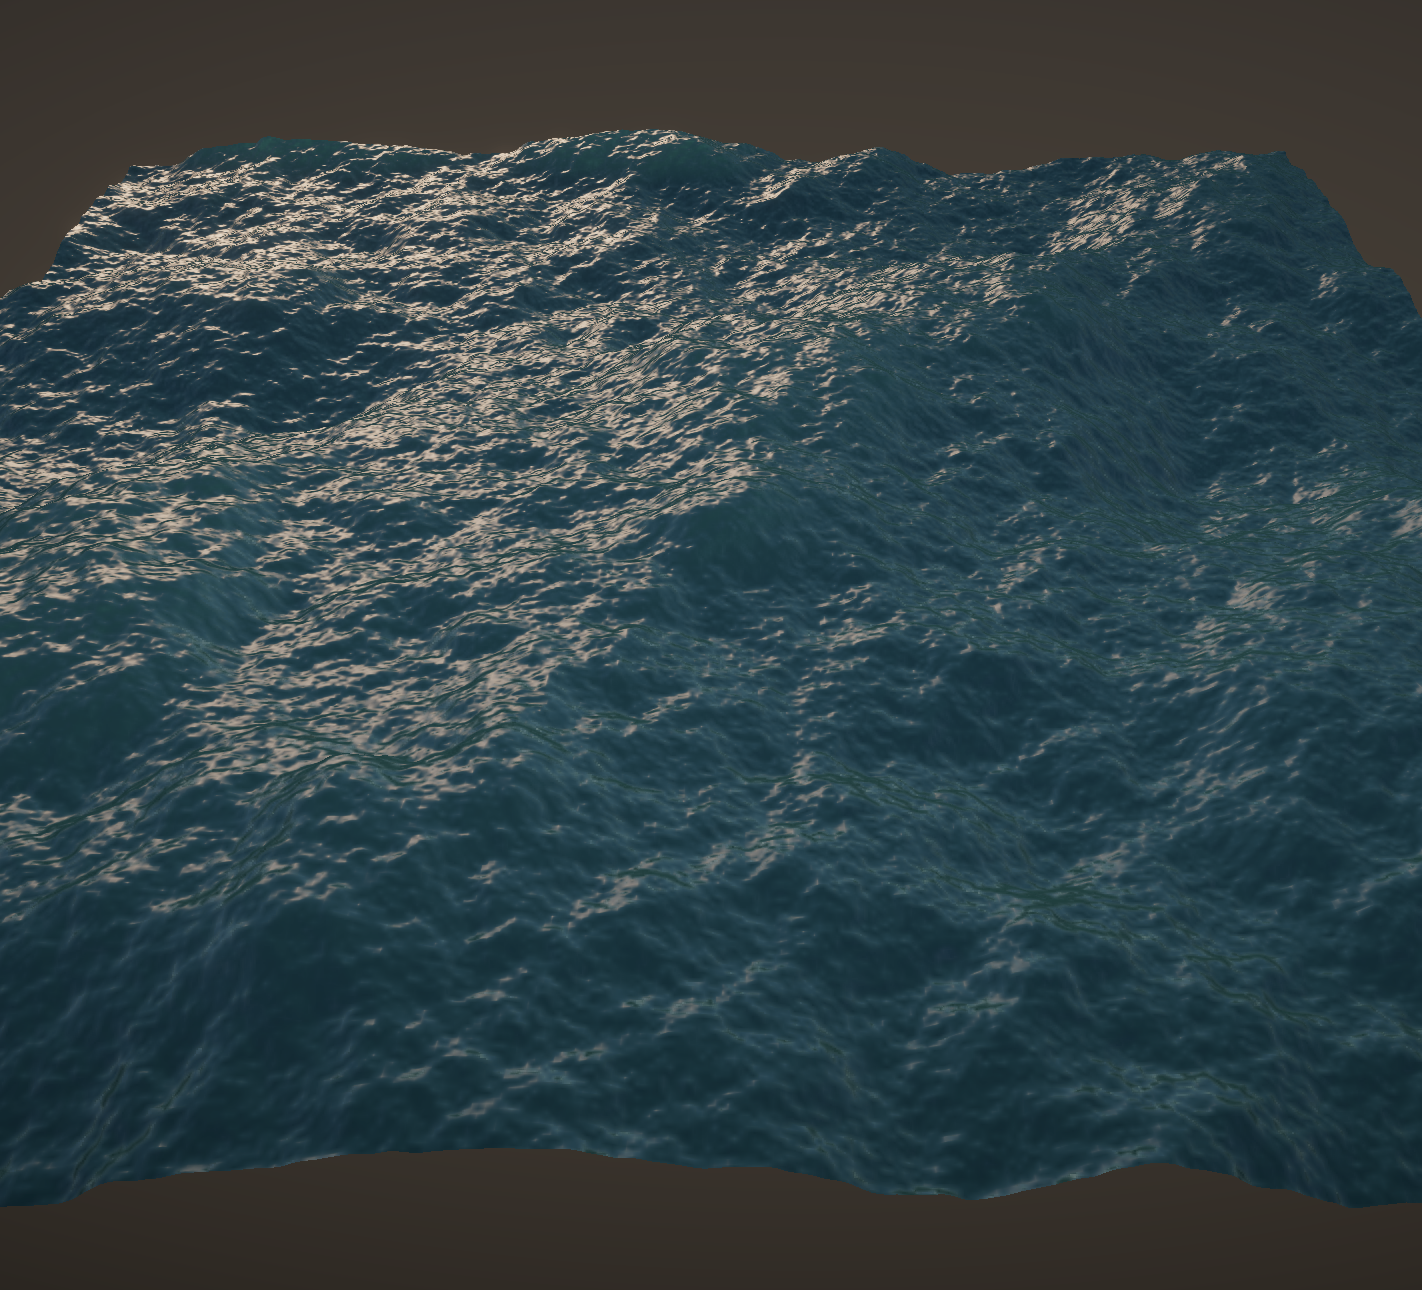
\includegraphics[width=0.40\textwidth]{"images/rendered_height_no_coppy.png"}
    \captionof{figure}{Ocean without Choppy Waves}
    \label{fig:ocean_no_choppy}
\end{minipage}

To make waves choppy we need to introduce horizotal displacement. This will not only make waves more chopy but also make energy transfer between waves more relistic. Following formula from \cite[J. Tessendorf]{tessendorf2004} we can calculate horizontal displacement:
\begin{equation}
    D_{\text{hori}}(\textbf{x}, t) = -i\frac{\mathbf{k}}{k}\tilde{h(\mathbf{k}, t)}
\end{equation}
Once again we need to perform IFFT \ref{fig:ifft_algorithm} to get horizontal displacement in the time domain.

\begin{minipage}{1\textwidth}
    \centering
    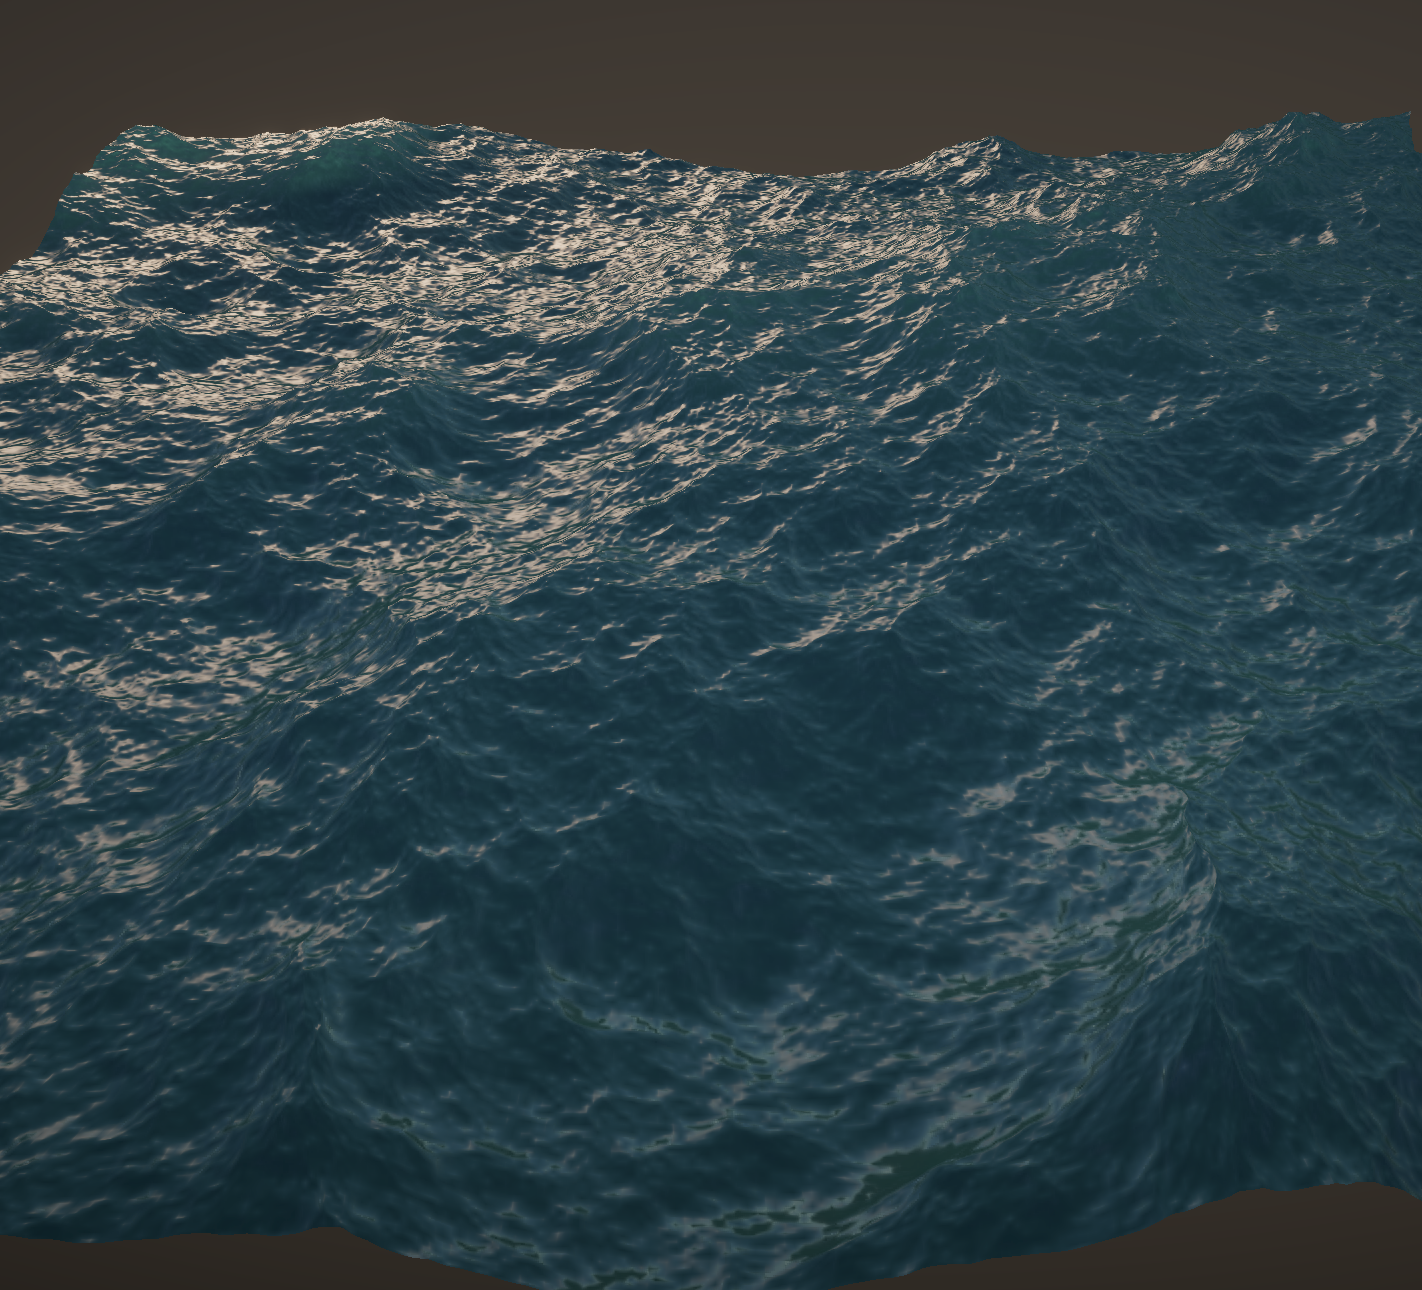
\includegraphics[width=0.40\textwidth]{"images/rendered_height_choppy.png"}
    \captionof{figure}{Ocean with Choppy Waves}
    \label{fig:ocean_choppy}
\end{minipage}

\section{Ocean Shading}

\begin{table}[H]
    \centering
    \begin{tabular}{|c|c|c|}
        \hline
        \textbf{Symbol} & \textbf{Parameter} \\
        \hline
        $L_A$ & Ambient Light \\
        \hline
        $N$ & Normal \\
        \hline
        $D_V$ & View Direction \\
        \hline
        $C_A$ & Ambient Light Color \\
        \hline
        $C_L$ & Light Color \\
        \hline
        $C_B$ & Air Bubble Color \\
        \hline
        $F$ & Fresnel Effect \\
        \hline
        $\rho_a$ & Air Bubble Density \\
        \hline
        $k_A$ & Ambient Light Intensity \\
        \hline
    \end{tabular}
    \caption{Lighting Parameters}
    \label{table:lighting_parameters}
\end{table}

\subsection{Lighting}

\subsubsection{Ambient Light}
Ambient light is light that does not come from any specific light source, but rather result of light being scattered in the environment. It is constant and does not depend on the direction of the light source.
For ocean we use  ambient light aproximation formula taken from GDC confference \cite{mark2021}:
\begin{equation}
    L_A = k_A N C_A C_L + \rho_a C_B C_L
\end{equation}

\subsubsection{Fresnel Effect}
Fresnel effect is the phenomenon where light is more reflective at grazing angles. This effect will be importatnt for specular and reflection calculations.
Approximation formula ctakes form of:
\begin{equation}
    F = (1 - \max(D_V \cdot N, 0.15))^{5}
\end{equation}

\subsubsection{Subsurface Scattering}
\begin{equation}
    \begin{split}
        L_S &= (L_S1 + L_S2) C_{WS} C_L\\
        L_S1 &= k_S1 \max(0, H) ([D_S, -D_V])^{4}(0.5-0.5(D_s \cdot N))^{3}\\
        L_S2 &= k_S2 ([D_V, N])^{2}
    \end{split}
\end{equation}

\subsubsection{Specular Reflection}

\subsubsection{Reflection}

\subsubsection{Output}

\subsection{Foam}

% Before we start, all callculations were taken inside GPU, using HLSL language. This allows us to use parallelism and speed up the process dramatically.
% As FFT requires our sample data length be power of 2, we will use $n \cdot n = 512 \text{x} 512$ textures to represent our data.

% \section{Spectrum Generation}
% \subsection{Tessendorf Spectrum}
% To generate height map \ref{eq:height_map} for our ocean we firstly need to generate spectrum. Firstlly, I chose to use J. Tessendorf's spectrum model \ref{eq:tessendorf_spectrum} as this was straight forward to implement:
% $$
% P_h(\mathbf{k}) = A \frac{e^{-1/(kl)^{2}}}{k^{4}}| \mathbf{\hat{k}} \cdot \mathbf{w} |^{6}
% $$
% where $\mathbf{k} = (k.x, k.y)$, $k.x = 2 * \pi (x.x - n/2)/ l$, $k.y = 2 * \pi (x.y - n/2)/ l$, $l$ is the the length scale of the ocean, 
% anx $\mathbf{x} = (x.x, x.y)$ is current position in the texture. 

% \subsection{TMA Spectrum}
% However, this model was not perfect, as it produced waves that didn't seem to transfer energy in the right way and the waves didn't seem to follow wave dircetion.
% Therefore, I decided to use JONSWAP spectrum with TMA correction that was suggested by \cite{horvath2015} \ref{eq:tma_spectrum}, however in our case $h$ will be constant therefore we can rewrite the function as:
% \begin{equation}
%     S_{TMA}(\omega) = S_{JONSWAP}(\omega) \cdot S_{TMA}(\omega)    
% \end{equation}
% Currentlly, we have two problems with this equation. Firstlly, this spectrum is non-directional, so we need to add directionality to it. Secondly, 
% this spectrum accepts $\omega$ as input, but as we following J. Tessendorf's \cite{tessendorf2001} paper, we need to use $\mathbf{k}$ as input. 

% \subsection{Directional Spectrum}



% According earlier expressed equation \ref{eq:height_map} we use DFT to calculate height map. Because we going to use FFT we can remove the exponential part as this will be calculated inside FFT algorithm:
% \begin{equation}
%     h(\mathbf{x}) = \sum_{\mathbf{k}} \tilde{h}(\mathbf{k}, t)
% \end{equation}
% , we can see that fft-based representation expresses ocean height at horizontal plane $\mathbf{x} = (x, y)$ "as the sum of sinusoids with complex, time-dependent amplitudes"\cite{tessendorf2001}.
% where, $\mathbf{k} = 2\pi $
